% ---------------------------------------------------------------------------
% Author guideline and sample document for EG publication using LaTeX2e input
% D.Fellner, v1.13, Nov 13, 2007

\documentclass{egpubl}
\usepackage{SIACG09}

% --- for  Annual CONFERENCE
%\ConferenceSubmission % uncomment for Conference submission
 %\ConferencePaper      % uncomment for (final) Conference Paper
% \STAR                 % uncomment for STAR contribution
% \Tutorial             % uncomment for Tutorial contribution
% \ShortPresentation    % uncomment for (final) Short Conference Presentation
%
% --- for  CGF Journal
% \JournalSubmission    % uncomment for submission to Computer Graphics Forum
% \JournalPaper         % uncomment for final version of Journal Paper
%
% --- for  CGF Journal: special issue
% \SpecialIssueSubmission    % uncomment for submission to Computer Graphics Forum, special issue
% \SpecialIssuePaper         % uncomment for final version of Journal Paper, special issue
%
% --- for  EG Workshop Proceedings
\WsSubmission    % uncomment for submission to EG Workshop
% \WsPaper         % uncomment for final version of EG Workshop contribution
%
 \electronicVersion % can be used both for the printed and electronic version

% !! *please* don't change anything above
% !! unless you REALLY know what you are doing
% ------------------------------------------------------------------------

% for including postscript figures
% mind: package option 'draft' will replace PS figure by a filname within a frame
\ifpdf \usepackage[pdftex]{graphicx} \pdfcompresslevel=9
\else \usepackage[dvips]{graphicx} \fi

\PrintedOrElectronic

% prepare for electronic version of your document
\usepackage{t1enc,dfadobe}

\usepackage{egweblnk}
\usepackage{cite}

% For backwards compatibility to old LaTeX type font selection.
% Uncomment if your document adheres to LaTeX2e recommendations.
\let\rm=\rmfamily    \let\sf=\sffamily    \let\tt=\ttfamily
\let\it=\itshape     \let\sl=\slshape     \let\sc=\scshape
\let\bf=\bfseries

% end of prologue

% ---------------------------------------------------------------------
% EG author guidelines plus sample file for EG publication using LaTeX2e input
% D.Fellner, v1.12, Oct 21, 2005


%\title[Building OBB Trees using Genetic Algorithms for Collision Detection]%
%      {Building OBB Trees using Genetic Algorithms for Collision Detection}
\title[Optimizing Collision Detection based on OBB Trees Generated with GA]%
      {Optimizing Collision Detection based on OBB Trees Generated with Genetic Algorithm}

% for anonymous conference submission please enter your SUBMISSION ID
% instead of the author's name (and leave the affiliation blank) !!
\author[E. Ram\'irez, H. Navarro, R. Carmona \& A. Dos Ramos]
       {E. Ram\'irez$^1$, H. Navarro$^{1}$, R. Carmona$^{1}$
        and J. Dos Ramos$^{1}$
%        S. Spencer$^2$ 
        \\
         $^1$CCG, Universidad Central de Venezuela\\
%        $^2$ Another Department to illustrate the use in papers from authors
%             with different affiliations
       }

% ------------------------------------------------------------------------

% if the Editors-in-Chief have given you the data, you may uncomment
% the following five lines and insert it here
%
% \volume{23}   % the volume in which the issue will be published;
% \issue{2}     % the issue number of the publication
% \pStartPage{201}      % set starting page


%-------------------------------------------------------------------------
\begin{document}

\maketitle

\begin{abstract}

In this paper a method for generating Oriented Bounding Boxes (OBB) using genetic algorithms (GA) is proposed. OBBs are used in a hierarchy of bounding volumes to detect collisions between objects. Currently, the most used method  for generating OBBs is based on the covariance matrix (CV) of the points of the model, but it has many flaws and in most cases does not find the optimum OBB. We performed several tests with both methods (CV vs. GA). Generally the GA method provides a better adjustment of the OBB to the geometry of the models than the CV method. The metric used for measuring the adjustment of the OBB was the volume of the OBB. The time required for performing the collision detection was also tested, obtaining better results with the GA method. It is suggested to use the GA method when the models are rigid and will not be deformed.\\

\begin{classification} % according to http://www.acm.org/class/1998/
\CCScat{I.3.5}{Computer Graphics}{Object hierarchies}
\end{classification}

\end{abstract}

%-------------------------------------------------------------------------
\section{Introduction}

Collision detection is a very important field in computer graphics used for Virtual Reality applications, Video Games, Architectural Design Systems, Path-planning systems among others \cite{OBBTesis,Navarro}. There are several techniques for achieving collision detection \cite{COLL1},\cite{COLL2},\cite{COLL3},\cite{COLL4}. One of the most used group of collision detection techniques are hierarchical, based on a tree that subdivides objects \cite{TREE},\cite{AABBTREE} recursively. On each node of the tree there is a bounding volume (sphere, box, k-DOP, convex hull, etc.) that encloses all the triangles on that area. Two OBB trees can be searched simultaneously in order to check collisions, avoiding the need to test collisions between all triangles of the two models. One of the most used bounding volumes are Oriented Bounding Boxes (OBBs) \cite{Gottschalk96obb}, which are bounding boxes with specific orientations, instead of being aligned with the axis (Axis Aligned Bounding Boxes - AABBs), as can be seen in Figure \ref{fig:aabb_vs_obb}.

\begin{figure}[htb]
  \centering
  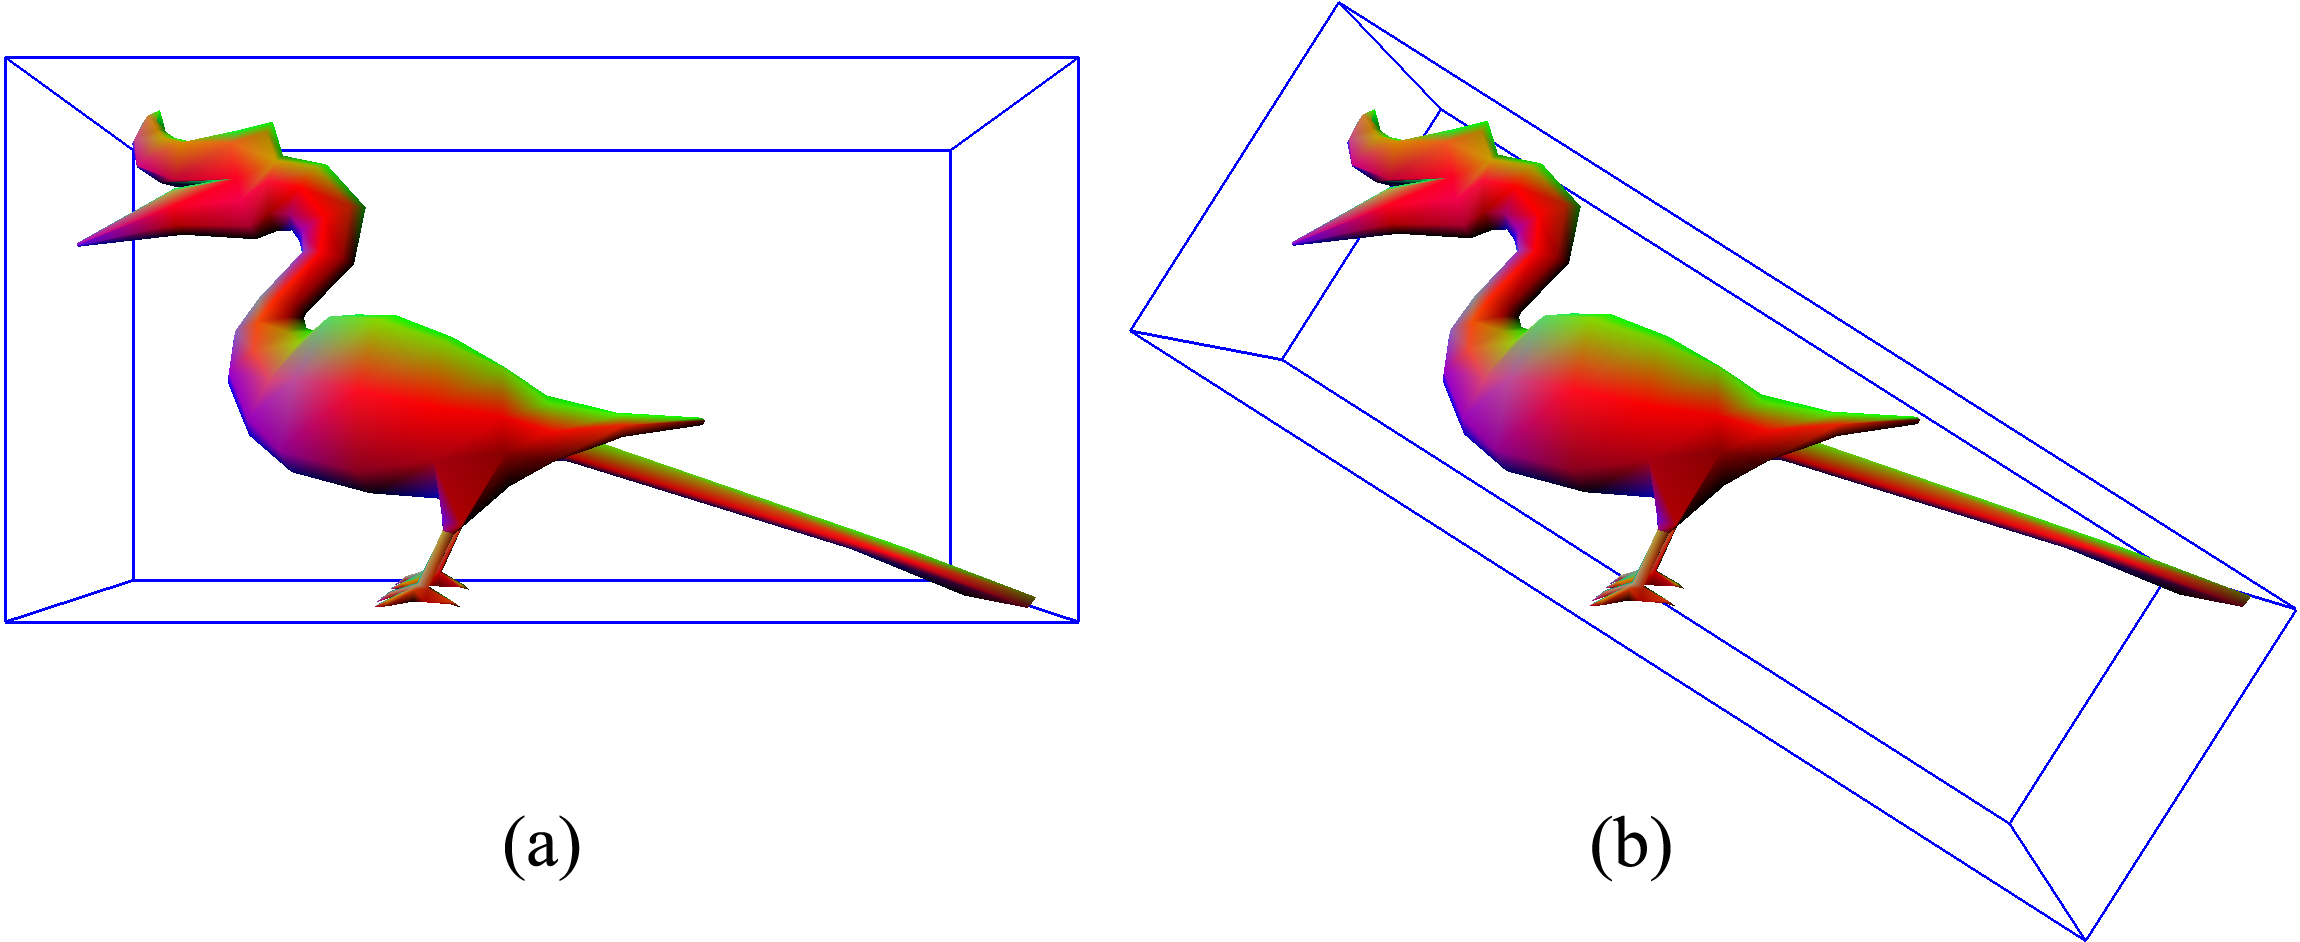
\includegraphics[width=.8\columnwidth]{images/ABBvsOBB}
  \caption{\label{fig:aabb_vs_obb}
           (a) AABB (b) OBB}
\end{figure}

OBBs are usually calculated by a statistical process that gives fast results at the expense of accuracy. The purpose of this work is to create a method for computing accurate OBBs, resulting in less required time for collision detection. Although the process of computing OBBs using genetic algorithms may be time consuming, this should be done only one time per object, storing the resulting OBB tree in a file for further use. The next section of this paper reviews related works. Next our implementation is described, followed by a discussion of the performed tests and the results we obtained. Lastly  conclusions are presented along with suggestions for future works in this field.

%-------------------------------------------------------------------------
\section{Background}

\subsection{Collision Detection}

In order to test for a collision, instead of checking collision between all pairs of triangles of the objects of interest, it is possible to check for collision between the bounding volumes. If the bounding volumes do not collide, then it is obvious that the triangles contended in them do not collide either. In case the bounding volumes collide one can go to the next level of the tree to check if the bounding volumes at that level collide. Figure \ref{fig:inCollision} shows a 2D example of this method. In the first level the bounding boxes intersect each other so collisions can not be discarded. On the next level the bounding boxes do not intersect and collisions are discarded. Then, the collide process will continue until:

\begin{itemize}
\item The detection is discarded because the bounding volumes do not collide.
\item At some point a leaf of the tree is reached, which cannot be decomposed anymore, so the triangles inside of that bounding volume must be checked individually. The size of the bounding volumes at this level should be very small, so only a few triangles are contained in each one.
\end{itemize}

\begin{figure}[htb]
  \centering
  
\includegraphics[width=1.0\columnwidth]{images/inCollision.png}
  \caption{\label{fig:inCollision}
Collision detection using OBB tree in 2D}
\end{figure}

\subsection{OBB Tree}

Once a method for building oriented bounding boxes is defined, a hierarchy of oriented bounding boxes is built. This can be done top-down or bottom-up. Generally the top-down approach is used, in which the oriented bounding box of the whole model is calculated. On the next step the bounding box is divided along a line perpendicular to one axis in order to obtain two new bounding boxes and each triangle of the model is classified according to the bounding box it belongs to (notice that some triangles that lie on the border between this two bounding boxes may belong to both). Now a new oriented bounding box most be created for the points belonging to each of the two bounding boxes previously created. This process continues until:

\begin{itemize}
\item The height of the tree has reached a certain level (in order to prevent the tree from growing too much).
\item The number of triangles on the bounding box is lower that a prefixed value (this  value should be kept low in order to minimize the number of triangle-triangle comparisons that have to be done when to leaves of the trees collide).
\item Triangles inside of the bounding box are not divisible along any axis. Some implementations might try to divide the bounding box along the longest axis, some other implementations try to divide it along all axis.
\end{itemize}

Figure \ref{fig:trees} shows several steps on the creation of an oriented bounding box tree. Only the bounding boxes of the leaves are shown. As the tree gets refined, the union of the leves gets tighter to the model.\\

\begin{figure}[htb]
  \centering
  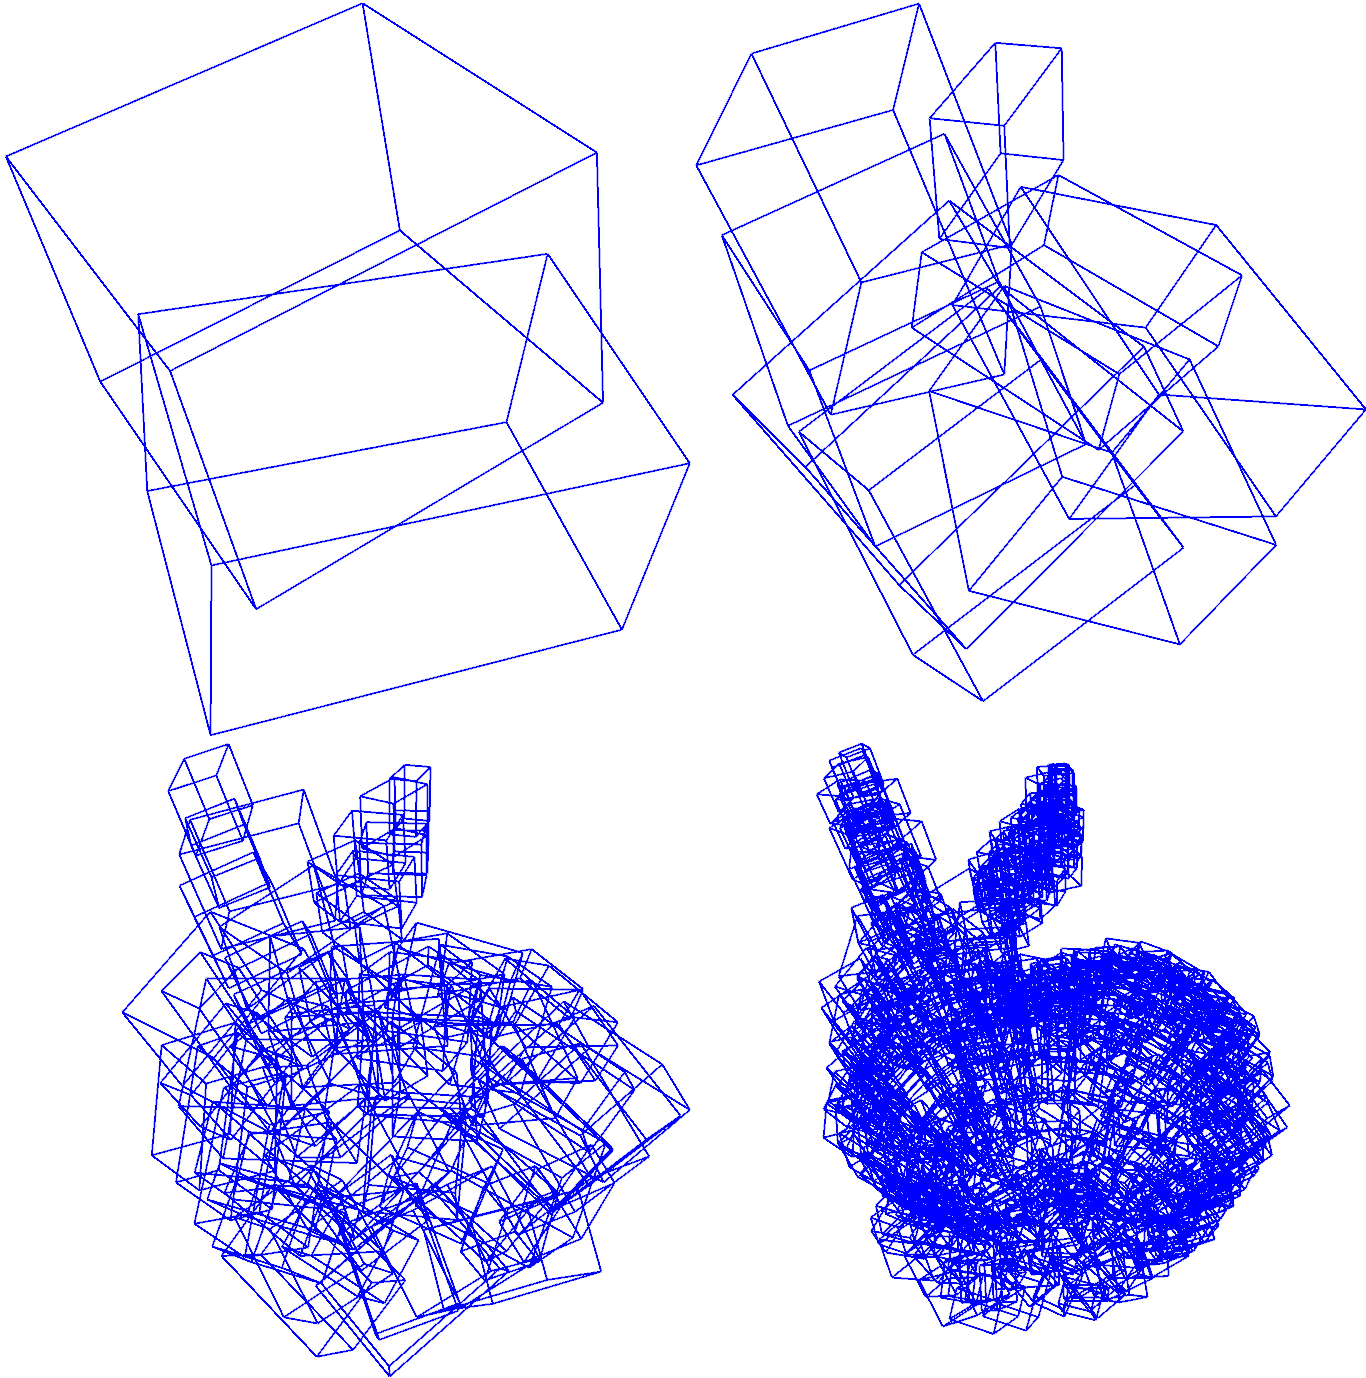
\includegraphics[width=1.0\columnwidth]{images/obbtree.png}
  \caption{\label{fig:trees}
           Steps on the creation of an OBB Tree. In the first step (top-left) the mesh has been divided in two groups whose OBBs are shown. Each step refines the OBBs, obtaining at the end a group of OBBs that resembles the original mesh. In this case the original mesh is Stanford bunny \cite{BUNNY}}
\end{figure}

Some desirable features of OBB trees are:

\begin{itemize}
\item The number of triangles ($N$) on each leaf should be minimal. When the collision detection is being performed, if two leaves intersect each other, it is necessary to check if any triangle of one leaf intersect with a triangle of the other leaf, leading to a $O(N^2)$ algorithm (depending on the number of triangles on the leaves).
\item The tree should be as balanced as possible in order to keep the collision of $O(N log_2(N))$.
\end{itemize}

Gottschalk et al. \cite{Gottschalk96obb} proposed a method for building OBBs out of a cloud of points. They state that the bounding box should fit the original model as tightly as possible. They propose to calculate the covariance matrix of the points and then its eigenvectors. The eigenvectors of this matrix are used as a basis for the oriented bounding box. The main drawback of this method is that internal points that should not influence the orientation of the object may change its orientation. One option to overcome this problem is to consider only the convex hull of the object using efficient and robust algorithms \cite{Gottschalk96obb}. However, if the convex hull has a very dense collection of points, there will be - again - an effect on the orientation of the OBB.

\subsection{Genetic Algorithms}

Genetic Algorithms (GA) \cite{Goldberg1989} are stochastic search methods that simulate the behavior of the natural biological evolution. Genetic algorithms work over a set of potential solutions applying the principle of the survival of the fittest and generate a better approximation of the solution. In each generation of individuals, a new set of approximations is created by the individual selection process according to their fitness value in the problem domain. This process continue until the individuals of the populations having the best performance into the environment can be survive, just like the naturally adaptation.

GAs are particulizations of Evolutive Algorithms (EA) \cite{Back1996}, where the main function to evolution is a cross process. A EA is defined by:
\[
	EA = \{I,\phi, \alpha, \psi, s, i, \mu, \lambda\}
\]
where
\begin{enumerate}
	\item $I$ is the individual domain
	\item $\phi: I \rightarrow \Re$, put real values in the individuals and is a fitness function.
	\item $\alpha$ is a probabilistics operator's set, e.g. $\zeta:I^2 \rightarrow I$ is a operator that requires a combination, i.e. two parents are required to create a new individual, with $\zeta \in\alpha$.
	\item $\psi:I^{\mu} \rightarrow \mu$ generation transition function that describes the complete transformation process from population $P$ to another $P'$, through the application of the evolutive operators and selection, where $\mu \in N$ being $N$ the number of individuals. A space of individuals, $I^{\mu}$ goes to other space with $\mu$ again, $I^{\mu}$.
	\item $s:I^{\lambda} \rightarrow I^{\mu}$, selection operator that obtains $\mu$ individuals from $\lambda$ individuals, where $\lambda, \mu \in N$. A space of $\lambda$ individuals, $I^{\lambda}$ selects a $\mu$ individual space, $I^{\mu}$.
	\item $i:I^{\mu} \rightarrow (true,false)$ is a stop criteria to the EA.
\end{enumerate}

GAs model natural processes, such as natural selection, crossover, mutation, and migration. Figure \ref{fig:genetic} shows the structure of a simple genetic algorithm.

\begin{figure}[htb]
  \centering
  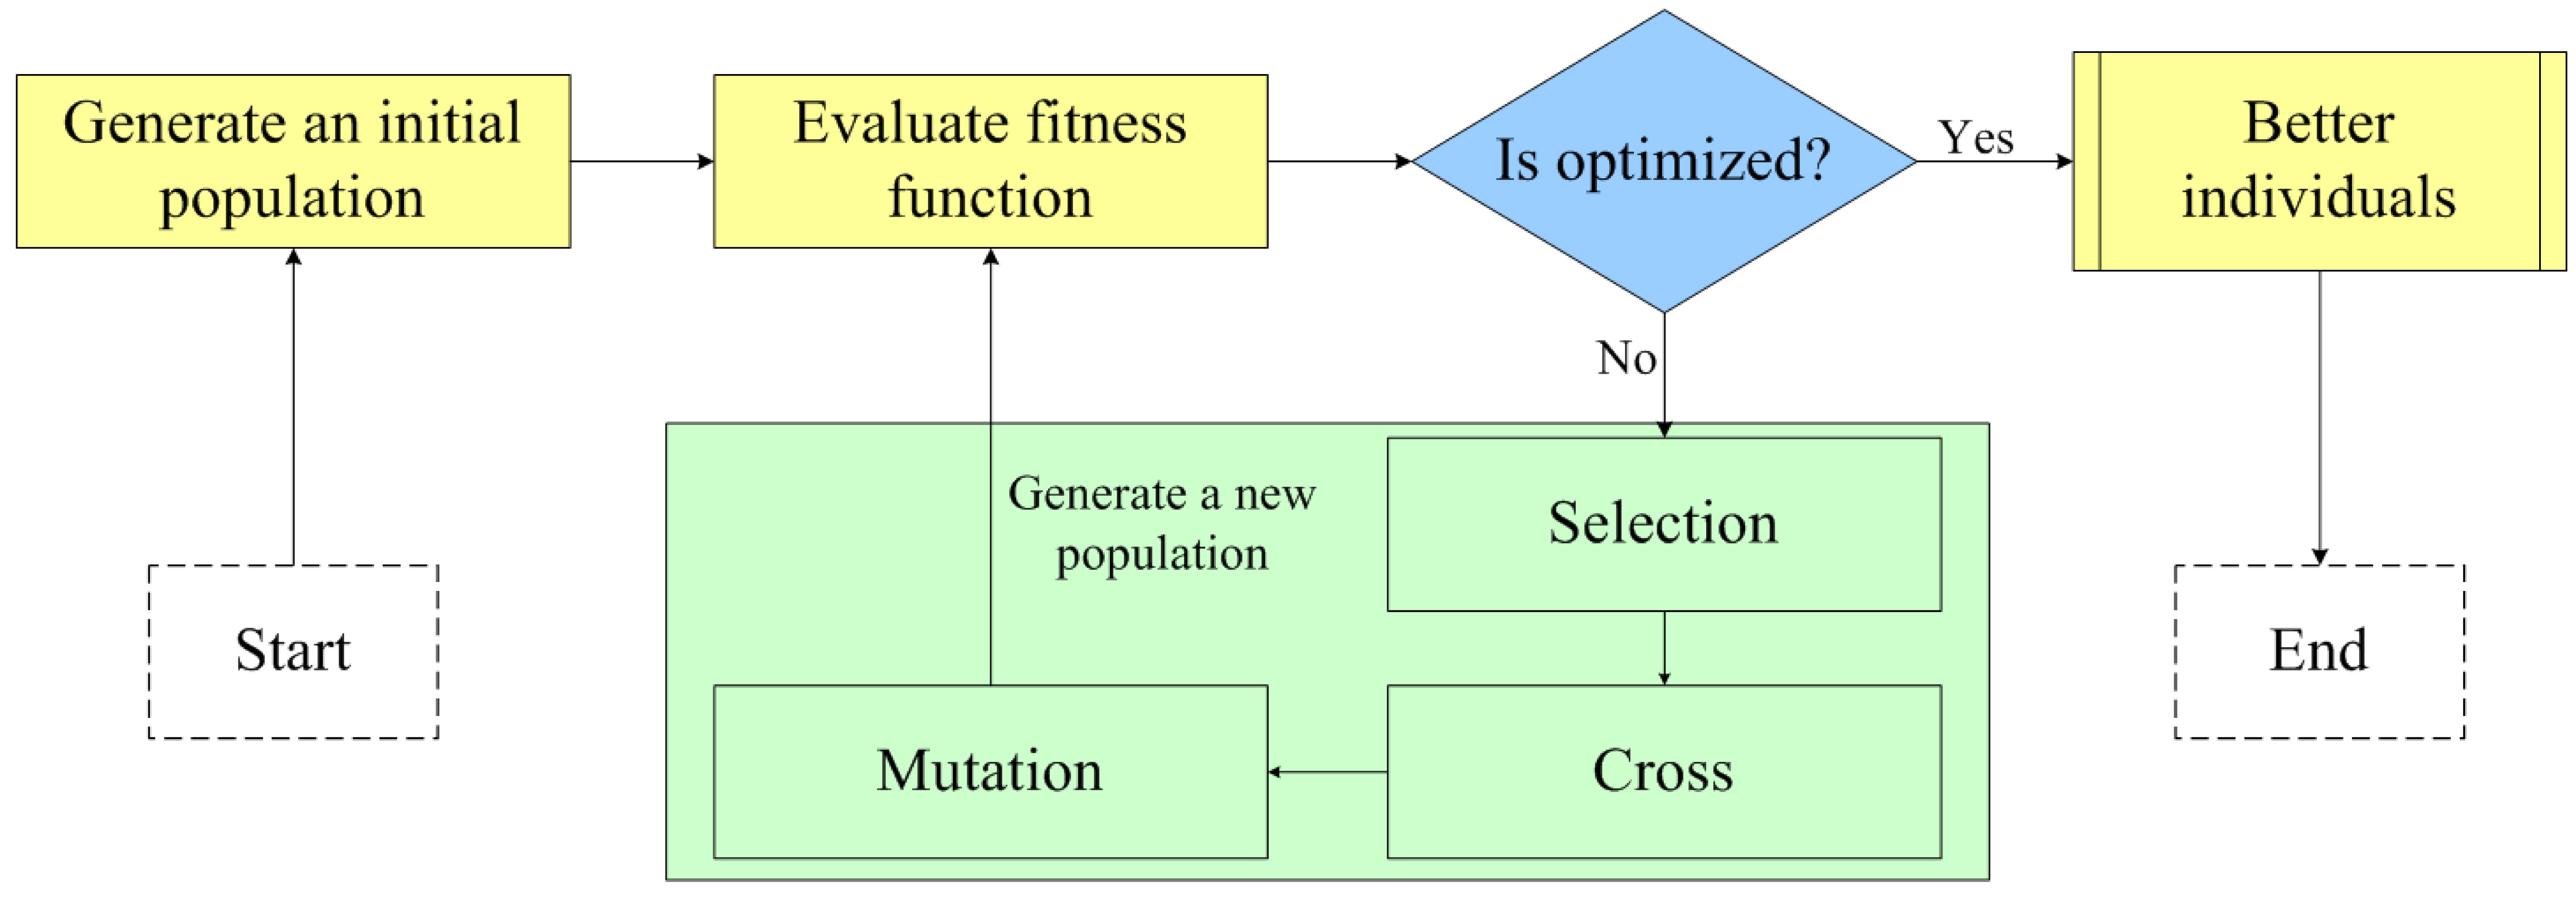
\includegraphics[width=1.0\columnwidth]{images/genetic.png}
  \caption{\label{fig:genetic}
           Genetic Algorithm process}
\end{figure}

In a GA at the beginning an initial population is created, which consists of a number of individuals which are potential solutions to the problem. Each of these individuals are given a fitness function that shows its quality with respect to the others. After evaluating individuals, there are individuals with a higher level of adaptation than others, which are better candidates to be a good solution. If the population is achieving optimal solution of the problem, then exists better individuals and therefore the solution. Otherwise, it applies a process of selection of individuals within the population; those individuals could be crossed (measured by a cross probability - CP) and obtain new individuals. It's also possible to apply any mutations (measured a mutation probability - MP) to individuals and thus achieve a new population which will be re-evaluated.

An individual corresponds with a chromosome, which is a data structure that encodes the parameters of a possible solution to the problem, a gene is a subsection of the chromosome. A chromosome is formed by alleles, that are the values that can take every possible position in the genetica. Each set of individuals is a generation, and a simple way of stopping the GA is by specifying a number of generations.

%-------------------------------------------------------------------------

\section{Implementation}

In this section we explain an implementation of our OBB tree created by genetic algorithm. We present the chromosomal representation, parameters of the genetic algorithm, and other implementation issues.

\subsection{Chromosomal Representation}

The oriented bounding boxes can be represented just specifying its orientation. Once the orientation is determined, the minimal bounding box that encloses the object can be easily computed. There are several ways to represent an orientation, but we decided to use quaternions \cite{GGII} because they are very compact and have important mathematical properties such as the absence of gimbal lock \cite{NASA}. A quaternion is a tuple $q=(x,y,z,w)$ which represents a rotation around an arbitrary axis. In order to represent a quaternion, we need then to represent four floating point values. The chromosomal is formed by 4 alleles, in Figure \ref{fig:chromosomal}, $(x,y,z)$ forms a vector and $w$ the rotation around the vector.

\begin{figure}[htb]
  \centering
  
\includegraphics[width=0.7\columnwidth]{images/chromosomal.png}
  \caption{\label{fig:chromosomal}
           Chromosomal Representation}
\end{figure}

The quaternion represents the rotation to apply in the three orthonormal vectors and assure the orthogonality condition. In our case the codification is binary and we used a 16 bit fixed representation for each of these values. That way, the range of values of each variable is divided in $2^{16}$ different values, e.g. if the range is [0,1], the values that can be represented are all multiple of $\frac{1}{2^{16}} \approx 1.52 x 10^{-5}$.

Figure \ref{fig:chromosomal_example} shows an example. Using 16 bits for each allele, the orientation vector $(x,y,z)$ takes the value $(44154,48625,47698)$ and the value of $w$ is $22935$. The next step is to normalize the values to the used range. The lower value for an orientation vector is $-1$ and the upper limit is $1$, then, the new value for $x$ would be $x'=-1+x*\frac{2}{2^{16}} \approx 0.3475$, $y'\approx0.4839$ and $z'\approx0.4556$. For $w$, the lower limit is $0$ and the upper is $360$ leading to $w'=w*\frac{360}{2^{16}}\approx262.0129$.


\begin{figure}[htb]
  \centering
  
\includegraphics[width=\columnwidth]{images/chromosomal_example.png}
  \caption{\label{fig:chromosomal_example}
           A chromosomal is formed by 8 bytes, 2 bytes per allele}
\end{figure}

\subsection{Parameters of the genetic algorithm}

Other important features of our genetic algorithm are:

\begin{itemize}
\item Generation Gap: the generation gap \cite{GA+DS=EP} is linked to the notion of non-overlapping and overlapping populations. In a non-overlapping model parents and offspring never compete with one another, i.e., the entire parent population is always replaced by the offspring population, while in an overlapping system, parents and offspring compete for survival. The generation gap refers to the amount of overlap between parents and offspring. In our implementation, the 20\% of the population is replaced (the worst individuals).
\item Fitness function: the fitness function is used to compare individuals in order to determine which one is fittest. In our case we consider that the best oriented bounding box is the one which fits the object more tightly. A good way for approximating this would be the volume of the bounding box. A lower volume means that the bounding box fits better the object. Since the fitness function is supposed to be higher for better individuals we decided to use $f = \frac{1}{V}$ where $V$ is the volume of the oriented bounding box.
\item Selection: the selection is the process that decides which individuals of the population will be crossed to obtain the next generation. We decided to use the roulette wheel method \cite{Goldberg1989} because it favors the fittest individuals and is very robust.
\item Cross over operator: The single point crossover operator has been selected on this work. The crossover operator will be applied with probability 0.8.
\item Mutation operator: the mutation operator will be random and applied with probability 0.03.
\item Generations: the max number of generations to be created is 150. This parameter worked properly for ours tests.
\end{itemize}

\subsection{Oriented Bounding Box}

As it was previously explained, the chromosomes represent a quaternion. If a chromosome encodes the quaternion $(x, y, z, w)$, then this quaternion is used to rotate the basis axes ($(1,0,0)$, $(0,1,0)$, $(0,0,1)$). Once the rotation is applied, three new axes are obtained ($\overrightarrow{A}, \overrightarrow{B}, \overrightarrow{C}$) which are the basis for creating an OBB. Now each point of the bounding box is projected into each of these axes in order to determine the major axis (the longest axis), see Figure \ref{fig:comparision}, and the start/finish points of each axis. The volume of OBB Figure \ref{fig:comparision}A is greater than the volume of OBB in Figure \ref{fig:comparision}B.

\begin{figure}[htb]
  \centering
  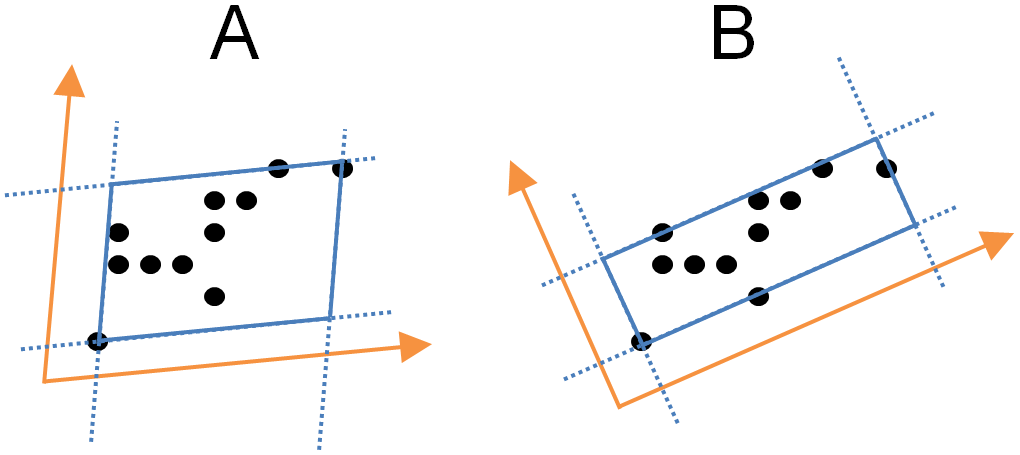
\includegraphics[width=\columnwidth]{images/comparision.png}
  \caption{\label{fig:comparision}
           2D example comparing the resulting bounding box using different rotations}
\end{figure}

Using these values, the center of the oriented bounding box is calculated, as well as the length of each side. The longest axis is used to split the bounding box in two in order to continue building the OBB tree recursively.

%-------------------------------------------------------------------------
\section{Tests and Results}

In order to test the effectiveness of the proposed method, several tests were applied to the resulting OBBs. All tests where run in a computer with a Quad 2 Core 2.4 GHz processor and 4 GB of RAM.  The OBB trees for four different models were built using the GA method and compared against OBB trees built by using the covariance (CV) method. The four models can be seen in Figure \ref{fig:figuramodelos}. The geometric characteristics of the models are showing in Table \ref{table:models}.

\begin{figure}[htb]
\centering
   % an empty figure just consisting of the caption lines
   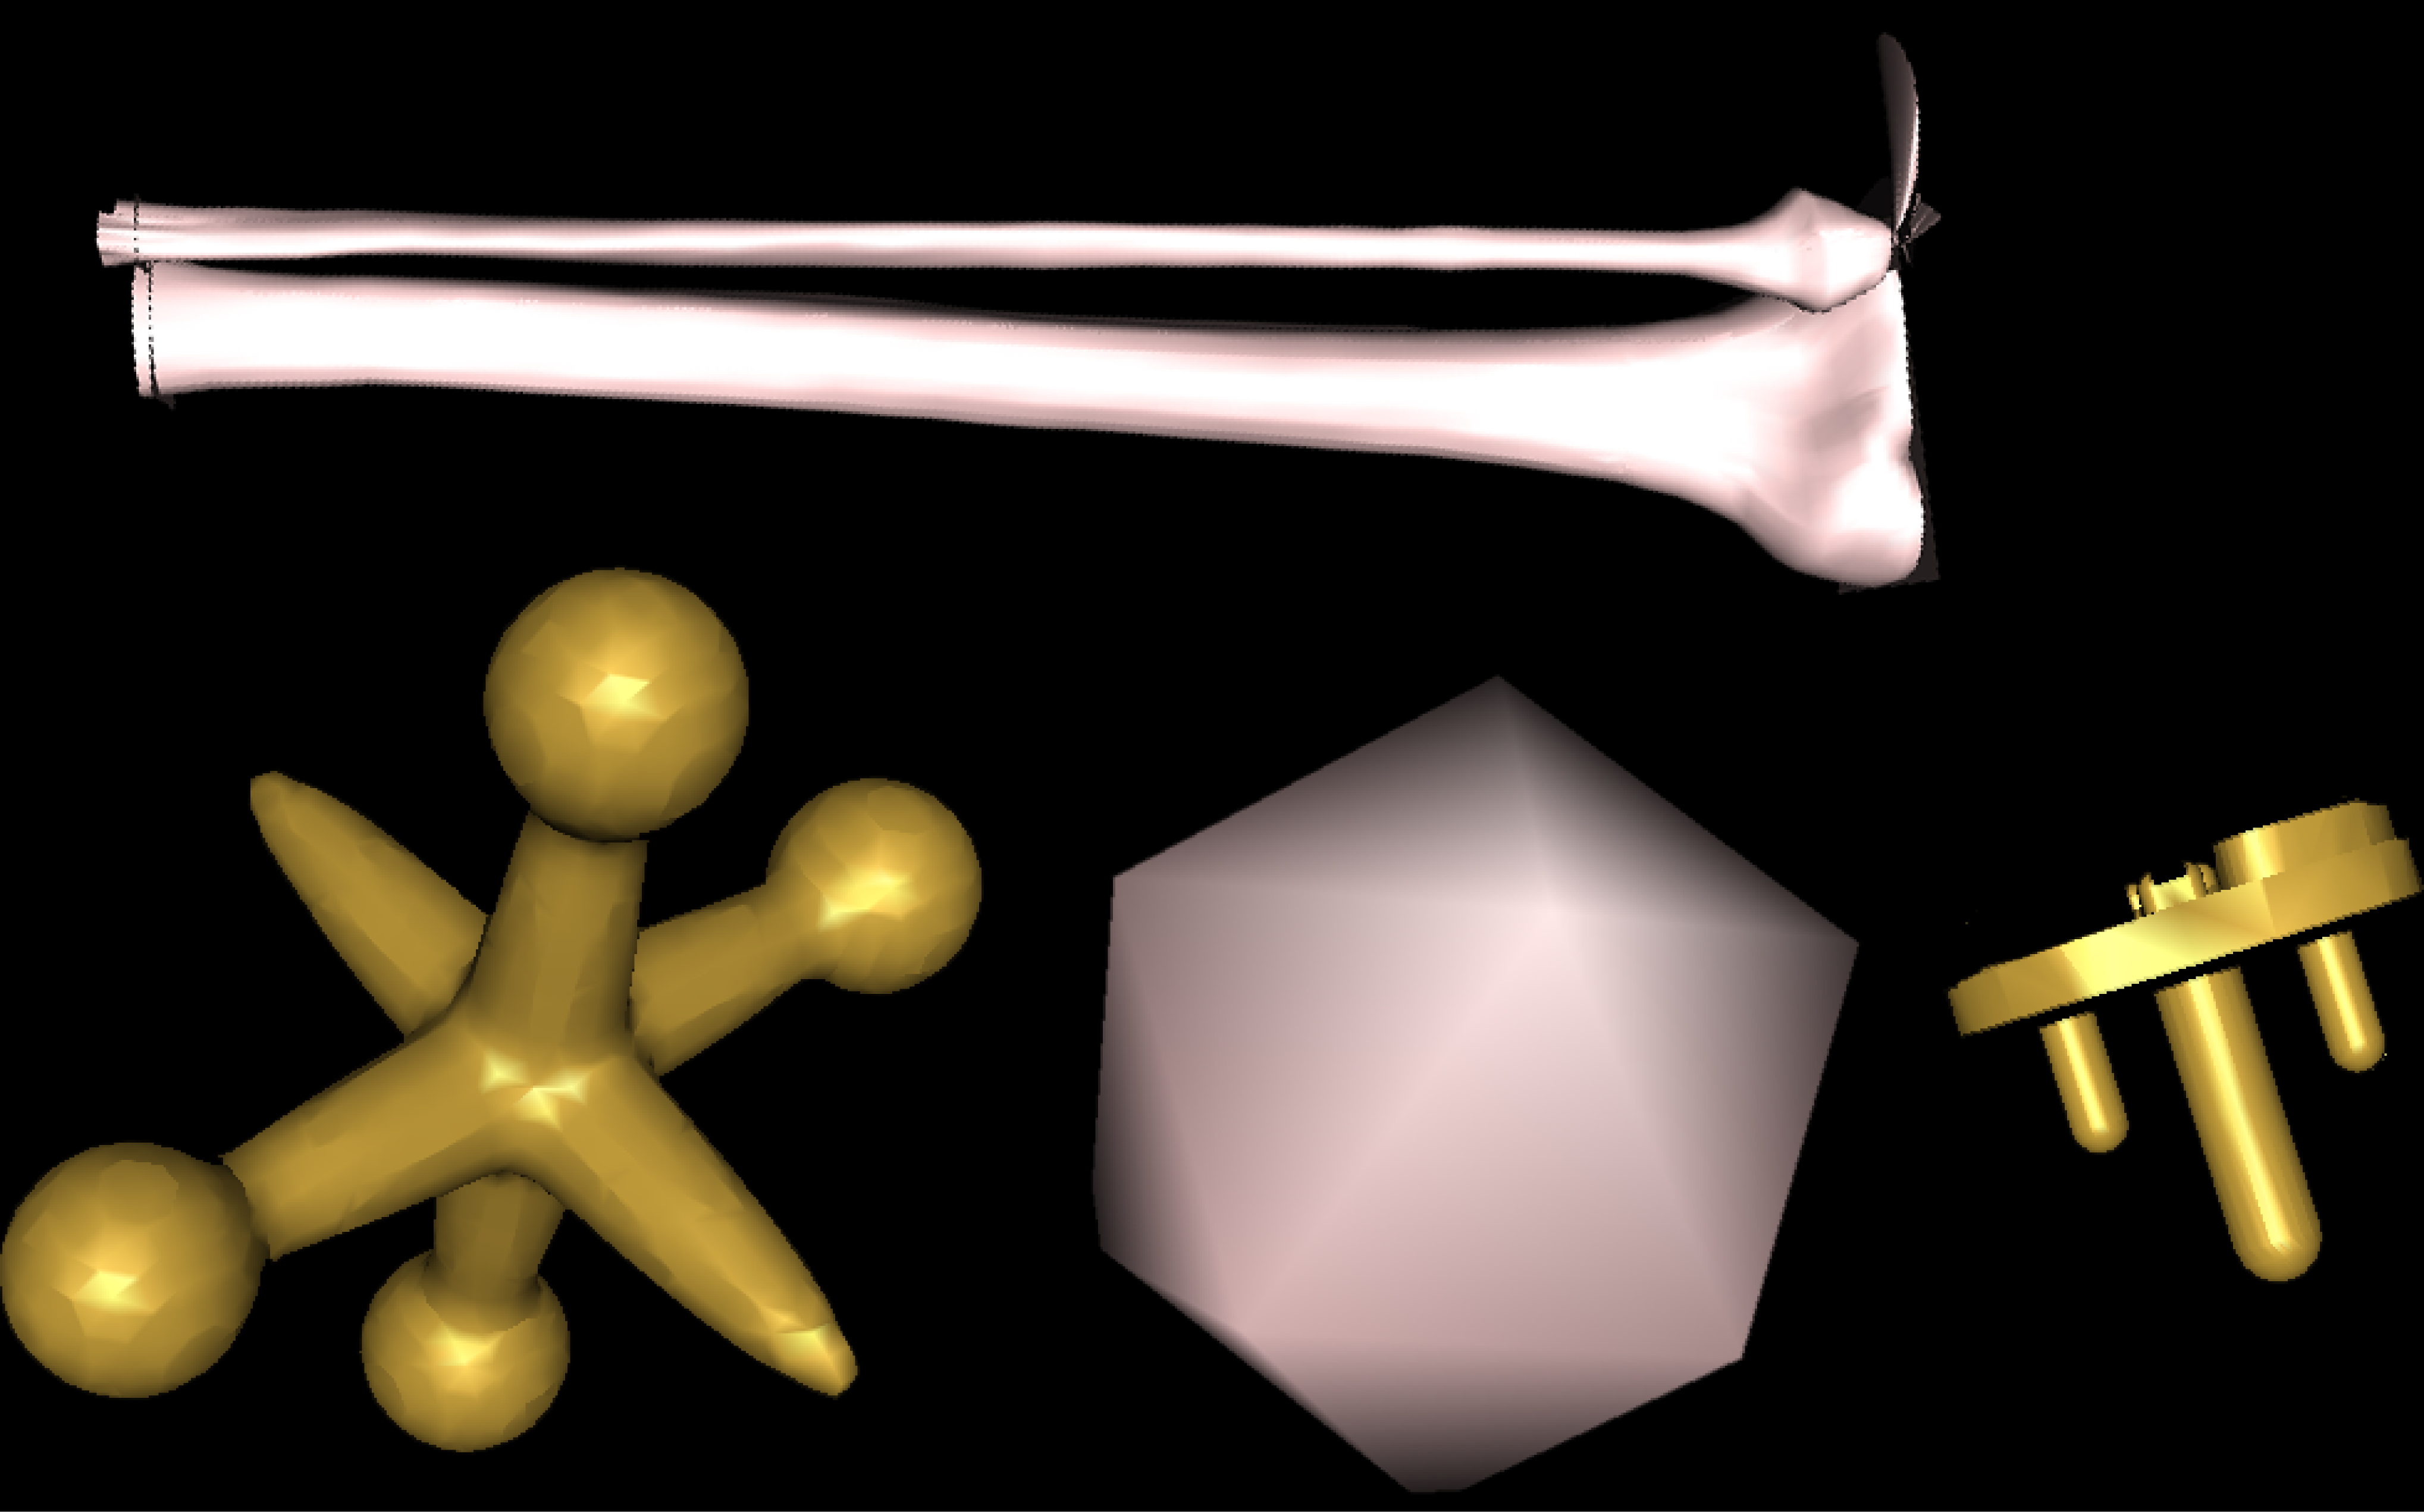
\includegraphics[width=0.9\columnwidth]{images/models.png}
   \caption{\label{fig:figuramodelos}
     Geometric models used for testing. In order of appearance (Top-bottom, left-right): tibia, jacky, sphere and prosthesis}
\end{figure}

\begin{table}[ht]
\caption{Testing models}
\centering
\begin{tabular}{c c c}
\hline \hline
% OJO AQUI ADAPTATION FUNCTION
Name & \# of Vertex & \# of Triangles\\ [0.75ex]
\hline
tibia & 7735 & 22662\\
jacky & 3304 & 6604\\
sphere & 12 & 20\\
prosthesis & 7252 & 9874\\ [1ex]\hline
\end{tabular}
\label{table:models}
\end{table}

Figure \ref{fig:Adaptation} shows the adaptation function for the GA in function of the generations, for the OBB of model \textit{tibia-(a)} and \textit{jacky-(b)}. It can be observed that the adaptation function grows as the number of generations increases. In Figure \ref{fig:Adaptation}A, from the 40th generation  (approximately) until the 150th, the adaptation function is almost constant for the consecutive generations. In Figure \ref{fig:Adaptation}B, the adaptation function is always growing, if the number of generations is higher then the feature will continue to grow to a point where it becomes constant. It is possible to decrement the number of generations to achieve faster results ($tibia$), but this could also interrupt the process of creating better individuals ($jacky$).

\begin{figure}[htb]
  \centering
  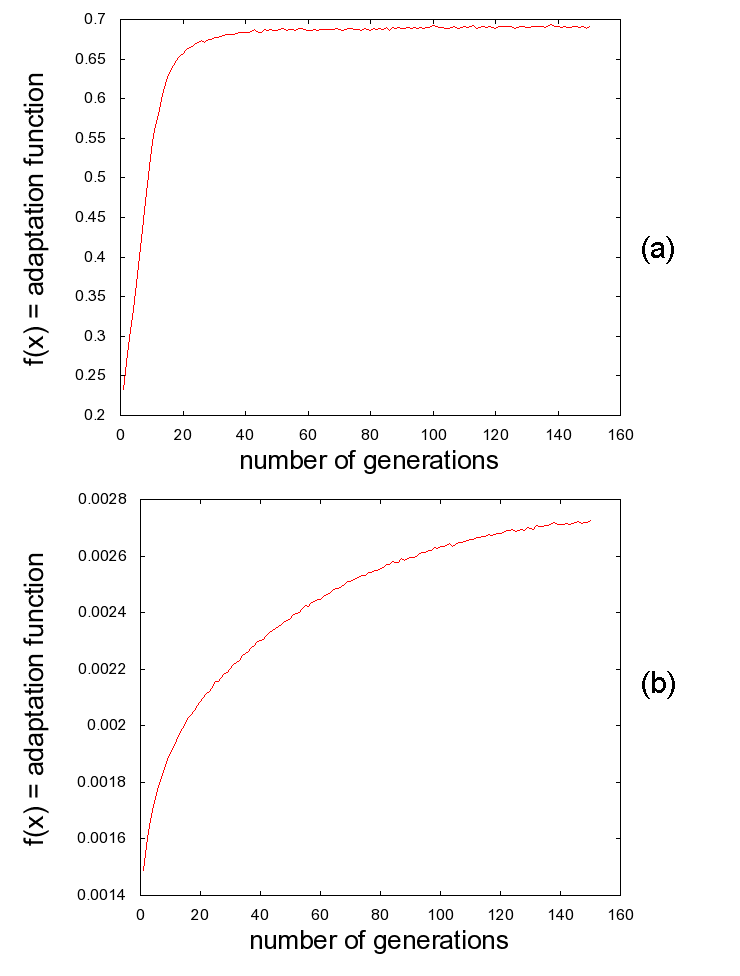
\includegraphics[width=0.9\columnwidth]{images/adaptation_gnuplot.png}
  \caption{\label{fig:Adaptation}
           Adaptation Function. (a) tibia (b) jacky}
\end{figure}

Table \ref{table:parameters} summarizes the parameters of our genetic algorithm, previously explained.

\begin{table}[ht]
\caption{Parameters for the GA}
\centering
\begin{tabular}{c c}
\hline \hline
Description & Value\\ [0.75ex]
\hline
Population & 100 individuals\\
Generations & 150\\
Cross Probability & 0.80\\
Mutation Probability & 0.03\\
Generational GAP & 20\%\\ [1ex]
\hline
\end{tabular}
\label{table:parameters}
\end{table}

As was previously explained, it is desirable that OBB trees minimize the number of triangles on each leaf. The next test was designed to measure this feature. Figure~\ref{fig:NTriangle} shows the average number of triangles per leaf on each one of the four models used. It can be seen that the GA method always gets lower average of triangles per leaf, although the difference on both methods is not too high.

\begin{figure}[htb]
  \centering
  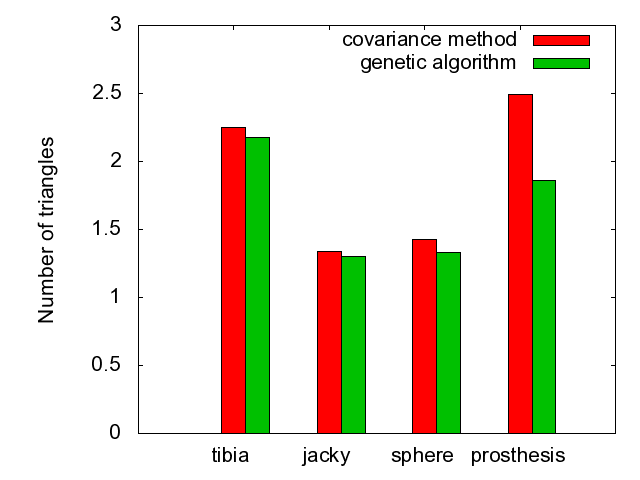
\includegraphics[width=1.0\columnwidth]{images/ntriangles}
  \caption{\label{fig:NTriangle}
           Average of triangles number per leaf}
\end{figure}

Using the previously described models several scenes were built, as described on Table \ref{table:scenes}.

\begin{table}[ht]
\caption{Description of the scenes. (Objects in the scene) and total number of triangle-triangle pairs (number of triangle-triangle intersections to test if no hierarchy is used)}
\centering
\begin{tabular}{c c c c}
\hline \hline
Scene & First object & Second object & Tri.-Tri. Pairs\\ [0.75ex]
\hline
1 & jacky & sphere & 132,080 \\
2 & jacky & tibia & 149,659,848 \\
3 & prosthesis & tibia & 223,764,588\\
4 & tibia & tibia & 513,566,244\\
\hline
\end{tabular}
\label{table:scenes}
\end{table}

The volume of the OBB is a good metric to measure the tightness of the bounding box. In the next test, the volume of the OBB of all leaves of the tree were added up for each model, using the CV and GA methods. Figure \ref{fig:volume} shows these volumes for each model. It can be observed that in all cases the GA method obtains better results (lower volumes). Table \ref{table:ninlin} shows the values for Figure \ref{fig:volume}.

\begin{table}[ht]
\caption{Volume}
\centering
\begin{tabular}{c c c }
\hline \hline
Case & Covariance & Genetic Algorithm \\ [0.75ex]
\hline
tibia & 3.462805 & 0.043980143 \\
jacky & 0.008262 & 0.000997286 \\
sphere & 0.581234 & 0.420012357 \\
prosthesis & 0.000023 & 0.000013521 \\  [1ex]
\hline
\end{tabular}
\label{table:ninlin}
\end{table}

\begin{figure}[htb]
  \centering
  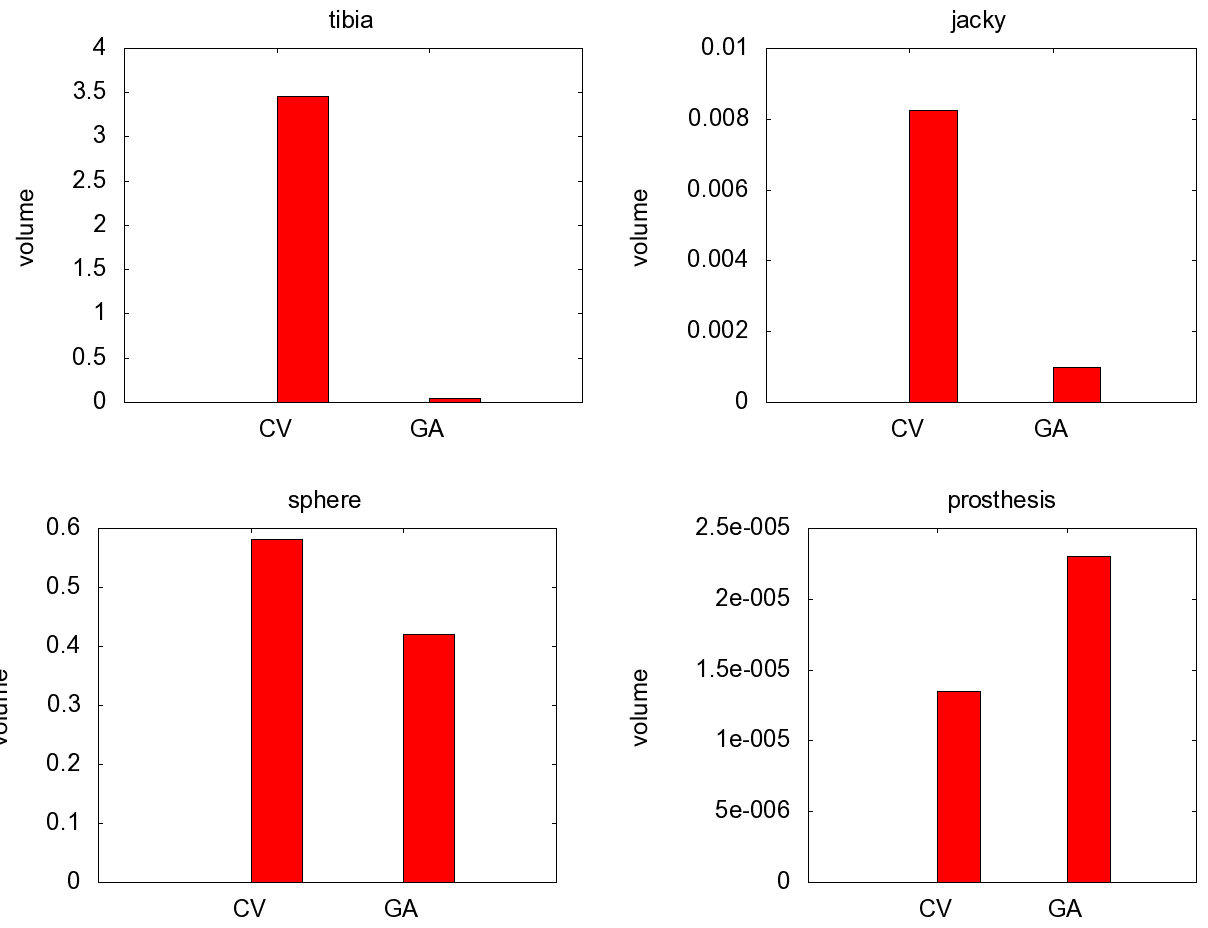
\includegraphics[width=1.0\columnwidth]{images/volumenes.png}
  \caption{\label{fig:volume}
Volume of the OBBs in the leaves}
\end{figure}

In order to check directly the influence of the OBB trees on the collision detection times, on each scene it was defined a path which consists of one object moving around the other object (sometimes touching it). On each step the collision detection time was evaluated and at the end the average collision detection times were taken. The results of this test are shown on Figure \ref{fig:Collide}. It can be seen that in all cases the average time required to perform collision detection using the GA method for the OBB's construction is less than CV method. In most cases the required time is about half.

\begin{figure}[htb]
  \centering
  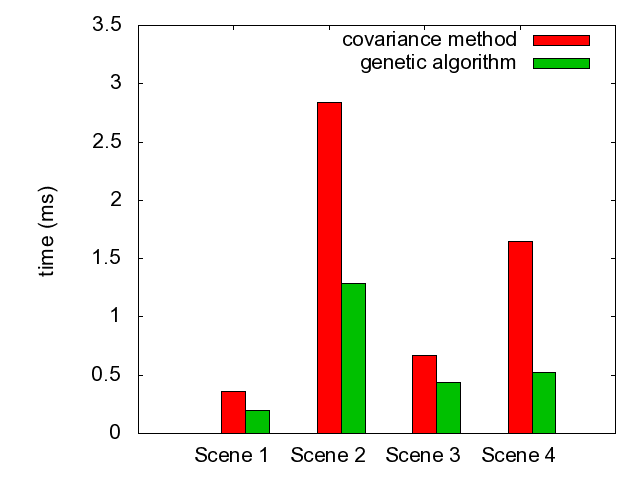
\includegraphics[width=1.0\columnwidth]{images/collide}
  \caption{\label{fig:Collide}
Average time for detecting collisions on each scene}
\end{figure}

Regarding times for building the OBB trees, Table \ref{table:times} shows the average times used for creating the trees for each model using the covariance method and the genetic algorithm. It is clear that the building times using the covariance method are lower, although for static objects, the OBB tree must be created one time, and it does not change on time. This is suitable for video games, virtual walkthroughs and several virtual reality applications.

\begin{table}
\caption{Time to build the OBBs using Covariance method and GA}
\centering
\begin{tabular}{c c c }
\hline \hline
Case & Covariance & Genetic Algorithm \\ [0.75ex]
\hline
tibia & 0.722060 sec. & 3070.33 sec. \\ % in second 3070.330620
jacky & 0.207357 sec. & 1036.32 sec. \\ % in second 1036.32
sphere & 0.196426 sec. & 3.204 sec. \\ %in minutes 0.053 min
prosthesis & 0.335531 sec. & 1657.01 sec. \\  %in second 1657.016
[1ex]
\hline
\end{tabular}
\label{table:times}
\end{table}

%-------------------------------------------------------------------------
\section{Conclusions and future works}

The genetic algorithm proposed for generating oriented bounding boxes achieves better results than the covariance method. The volume of the resulting oriented bounding boxes is lower, and the total time required for detecting collision between objects is also lower, in some cases reducing it in more than 68\%. If we take into account that collision detection is done on every frame, the gain is about 30ms per second (under a 30 frames per second basis) which can be used for other tasks such as simulation, rendering effects, artificial intelligence among others.\\

The genetic algorithm takes more time to build the OBB tree than the covariance method, but this has to be done only once, and the tree can be stored in a file for further uses. If the objects are to be deformed then the genetic algorithm can not be used.\\

The time for collision detection is closed related with the volume of the oriented bounding boxes. Methods for building OBBs should focus on fitting it as tight as possible.\\

We propose to study methods for recalculating the OBBs when the geometry of the model is slightly modified so the OBBs do not have to be totally recalculated. Another good application of genetic algorithms for computing OBB trees would be to allow the genetic algorithm to choose the axis along which each OBB will be divided on each level of the tree, instead of choosing the longest one as we did in this paper. This would lead to a global solution that should be better than the local solution that we are finding now.\\

It is suggested to use threads in both the genetic algorithm for generating the OBBs and the collision detection algorithm, in order to reduce the required time for these processes.\\

%-------------------------------------------------------------------------

\section*{Acknowledgment}
This research has been supported by the Scientific and Humanistic Development Council (Consejo de Desarrollo Cient�fico y Human�stico - CDCH) of the Central University of Venezuela (UCV), grant No. PG-03.00.65.2006.

\bibliographystyle{eg-alpha}
\bibliography{egbibsample}

\end{document}

